%%%%%%%%%%%%%%%%%%%%%%%%%%%%%%%%%%%%%%%%%%%%%%%%%%%%%%%%%%%%%%%%%%%%%%%%%%%%%%%%%%
\begin{frame}[fragile]\frametitle{}
\begin{center}
{\Large Data Types}
\end{center}
\end{frame}

%%%%%%%%%%%%%%%%%%%%%%%%%%%%%%%%%%%%%%%%%%%%%%%%%%%%%%%%%%%%%%%%%%%%%%%%%%%%%%%%%%%
\begin{frame}[fragile]\frametitle{Variables}

  \begin{itemize}
  \item A variable can be seen as a container (or some say a pigeonhole) to store certain values. 
  \item While the program is running, variables are accessed and sometimes changed, i.e. a new value will be assigned to a variable. 
    \item Every variable has and must have a unique data type.
  \item Declaring a variable means binding it to a data type.
  \item Defining a variable meas to have value assigned to it.
    \end{itemize}

\end{frame}

%%%%%%%%%%%%%%%%%%%%%%%%%%%%%%%%%%%%%%%%%%%%%%%%%%%%%%%%%%%%%%%%%%%%%%%%%%%%%%%%%%%
\begin{frame}[fragile]\frametitle{Variables in C/C++ or Java}
  \begin{columns}[c]
    \begin{column}{0.5\linewidth}
  \begin{lstlisting}
int x;
int y; 
\end{lstlisting}
  \begin{itemize}
  \item Such declarations make sure that the program reserves memory for two variables with the names x and y. 
  \item The variable names stand for the memory location. 
  \item It's like the two empty shoeboxes, labelled with x and y. 
  \item Like the two shoeboxes, the memory is empty as well.
    \end{itemize}
      \end{column}
    \begin{column}{0.4\linewidth}
    \begin{center}
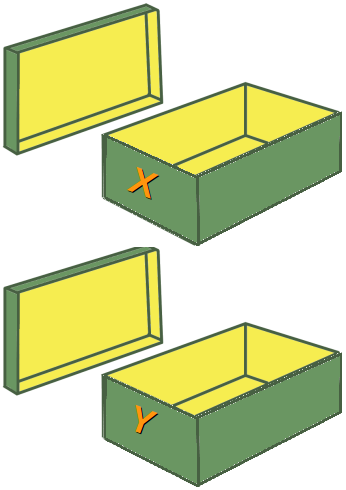
\includegraphics[width=0.3\linewidth,keepaspectratio]{boxes1}
\end{center}
        \end{column}
  \end{columns}
  
   % (Ref: https://www.python-course.eu/python3\_variables.php)
\end{frame}

%%%%%%%%%%%%%%%%%%%%%%%%%%%%%%%%%%%%%%%%%%%%%%%%%%%%%%%%%%%%%%%%%%%%%%%%%%%%%%%%%%%
\begin{frame}[fragile]\frametitle{Variables in C/C++ or Java}
  \begin{columns}[c]
    \begin{column}{0.5\linewidth}
  \begin{lstlisting}
x = 42;
y = 42; 
\end{lstlisting}
  \begin{itemize}
  \item Putting values into the variables can be realized with assignments. 
  \item Two numbers are physically saved in the memory, which correspond to the two shoeboxes.
    \end{itemize}
      \end{column}
    \begin{column}{0.4\linewidth}
    \begin{center}
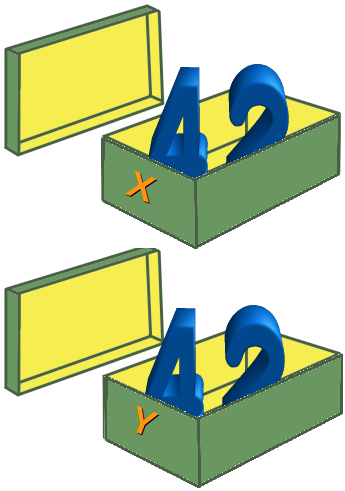
\includegraphics[width=0.3\linewidth,keepaspectratio]{boxes2}
\end{center}
        \end{column}
  \end{columns}
  
   % (Ref: https://www.python-course.eu/python3\_variables.php)
\end{frame}


%%%%%%%%%%%%%%%%%%%%%%%%%%%%%%%%%%%%%%%%%%%%%%%%%%%%%%%%%%%%%%%%%%%%%%%%%%%%%%%%%%%
\begin{frame}[fragile]\frametitle{Variables in C/C++ or Java}
  \begin{columns}[c]
    \begin{column}{0.5\linewidth}
  \begin{lstlisting}
y = 78;
\end{lstlisting}
  \begin{itemize}
  \item If we assign a new value to one of the variables, let's say the values 78 to y.
  \item We have exchanged the content of the memory location of y.

    \end{itemize}
      \end{column}
    \begin{column}{0.4\linewidth}
    \begin{center}
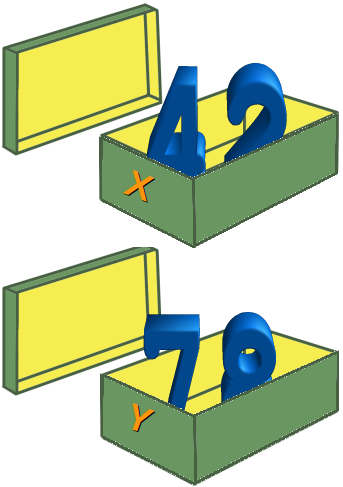
\includegraphics[width=0.3\linewidth,keepaspectratio]{boxes3}
\end{center}
        \end{column}
  \end{columns}
  
   % (Ref: https://www.python-course.eu/python3\_variables.php)
\end{frame}

%%%%%%%%%%%%%%%%%%%%%%%%%%%%%%%%%%%%%%%%%%%%%%%%%%%%%%%%%%%%%%%%%%%%%%%%%%%%%%%%%%%
\begin{frame}[fragile]\frametitle{Variables in Python}

  \begin{itemize}
  \item There is no declaration of variables required.
  \item Not only the value of a variable may change during program execution but the type as well.
\item You can assign an integer value to a variable, use it as an integer for a while and then assign a string to the same variable. 
    \end{itemize}

  \begin{lstlisting}
i = 42			# data type is implicitly set to integer
i = 42 + 0.11		# data type is changed to float
i = "forty"		# and now it will be a string  
\end{lstlisting}
  
   % (Ref: https://www.python-course.eu/python3\_variables.php)
\end{frame}


%%%%%%%%%%%%%%%%%%%%%%%%%%%%%%%%%%%%%%%%%%%%%%%%%%%%%%%%%%%%%%%%%%%%%%%%%%%%%%%%%%%
\begin{frame}[fragile]\frametitle{All variables in Python are references}
Python variables are references to objects, but the actual data is contained in the objects: 

    \begin{center}
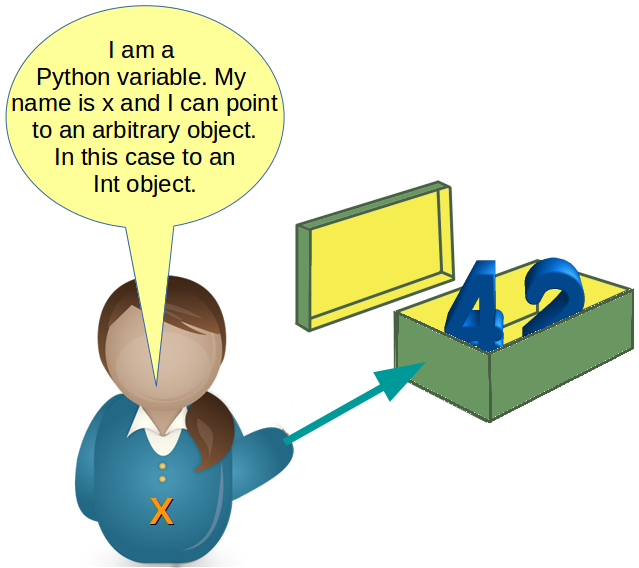
\includegraphics[width=0.5\linewidth,keepaspectratio]{boxes4}
\end{center}
  
  As variables are pointing to objects and objects can be of arbitrary data type, variables cannot have types associated with them.
  
   % (Ref: https://www.python-course.eu/python3\_variables.php)
   
   
\end{frame}


%%%%%%%%%%%%%%%%%%%%%%%%%%%%%%%%%%%%%%%%%%%%%%%%%%%%%%%%%%%%%%%%%%%%%%%%%%%%%%%%%%%
\begin{frame}[fragile]\frametitle{All variables are references}
\begin{lstlisting}
>>> x = 42
>>> y = x
\end{lstlisting}



    \begin{center}
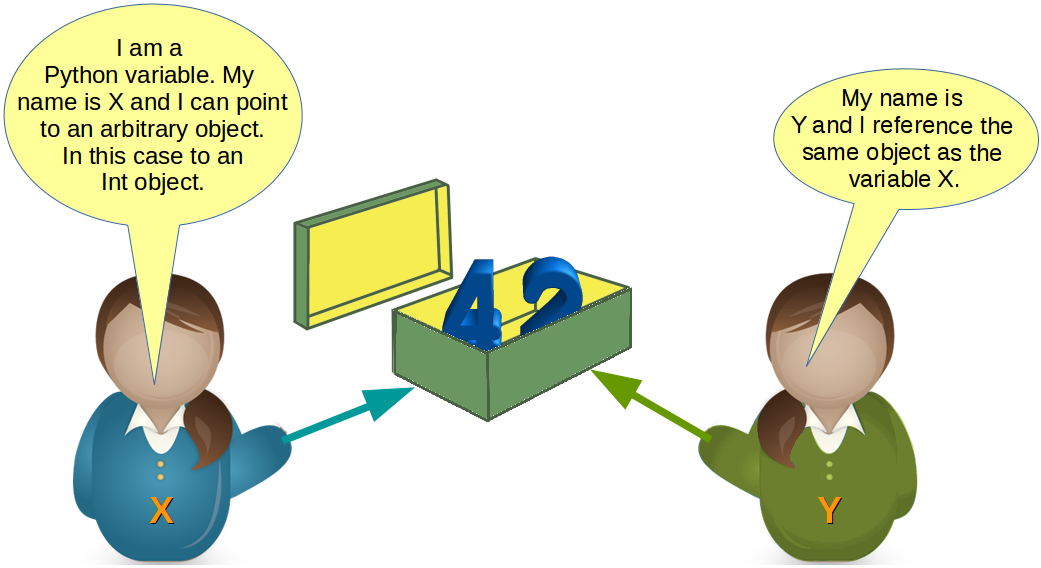
\includegraphics[width=0.5\linewidth,keepaspectratio]{boxes5}
\end{center}
  
  
   % (Ref: https://www.python-course.eu/python3\_variables.php)
   
   
\end{frame}



%%%%%%%%%%%%%%%%%%%%%%%%%%%%%%%%%%%%%%%%%%%%%%%%%%%%%%%%%%%%%%%%%%%%%%%%%%%%%%%%%%%
\begin{frame}[fragile]\frametitle{All variables are references}

What will happen, when we execute 

\begin{lstlisting}
y = 78
\end{lstlisting}
Python will create a new integer object with the content 78 and then the variable y will reference this newly created object, as we can see in the following picture: 


    \begin{center}
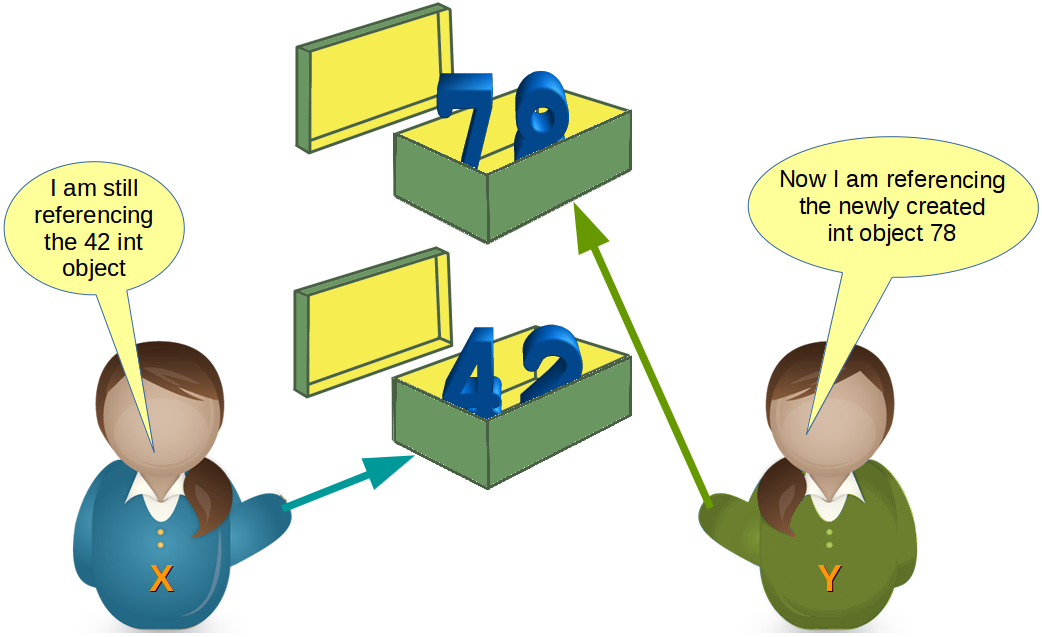
\includegraphics[width=0.5\linewidth,keepaspectratio]{boxes6}
\end{center}
  
  
   % (Ref: https://www.python-course.eu/python3\_variables.php)
   
   
\end{frame}


%%%%%%%%%%%%%%%%%%%%%%%%%%%%%%%%%%%%%%%%%%%%%%%%%%%%%%%%%%%%%%%%%%%%%%%%%%%%%%%%%%%
\begin{frame}[fragile]\frametitle{All variables are references}

What will happen, when we execute 

\begin{lstlisting}
x = ``Text''
\end{lstlisting}
The previously integer object "42" will be orphaned after this assignment. It will be removed by Python, because no other variable is referencing it. 


    \begin{center}
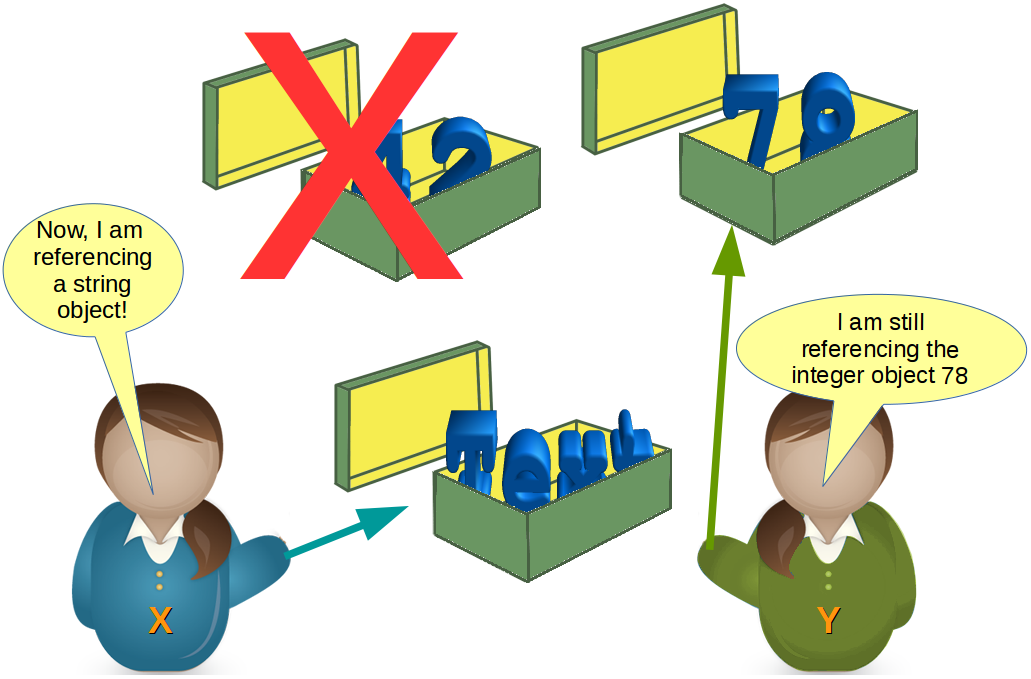
\includegraphics[width=0.5\linewidth,keepaspectratio]{boxes7}
\end{center}
  
  
   % (Ref: https://www.python-course.eu/python3\_variables.php)
   
   
\end{frame}


%%%%%%%%%%%%%%%%%%%%%%%%%%%%%%%%%%%%%%%%%%%%%%%%%%%%%%%%%%%%%%%%%%%%%%%%%%%%%%%%%%%
\begin{frame}[fragile]\frametitle{All variables are references}
In Python, \textbf{all objects are ever passed by reference}.
In particular, \textbf{variables always store a reference to an
    object}, never a copy!

  
  Hence, you have to be careful when modifying objects:
\begin{lstlisting}
>>> a = [1,2,3]
>>> b = a
>>> b.remove(2)
>>> print(a)
\end{lstlisting}

\emph{???}

\textbf{Q}: How many items are in the \texttt{a} list now?
%[1, 3]
\end{frame}


%%%%%%%%%%%%%%%%%%%%%%%%%%%%%%%%%%%%%%%%%%%%%%%%%%%%%%%%%%%%%%%%%%

 \begin{frame}[fragile]
   \frametitle{All variables are references}
   
However

 \begin{lstlisting}
 >>> a = 1
 >>> b = a
 >>> b += 1
 >>> a
 1
 >>> b
 2
 \end{lstlisting}

     How can you explain this?

     The $b += 1$ operator could be replaced by    $b = b + 1$, and the $b+1$ expression yields a
       new value.

 \end{frame}


%%%%%%%%%%%%%%%%%%%%%%%%%%%%%%%%%%%%%%%%%%%%%%%%%%%%%%%%%%%%%%%%%%%%%%%%%%%%%%%%%%%
\begin{frame}[fragile]\frametitle{Dynamic Typing: Python}
  \begin{itemize}
  \item Variables come into existence at first assignment.
  \item A variable can refer to an object of any type.
\item Can switch type based on assignment
  \item All types (almost) treated the same way.
  \item Type errors only caught in runtime.
    \end{itemize}

\end{frame}


%%%%%%%%%%%%%%%%%%%%%%%%%%%%%%%%%%%%%%%%%%%%%%%%%%%%%%%%%%%%%%%%%%%%%%%%%%%%%%%%%%%
\begin{frame}[fragile]\frametitle{Variables}
Definition-Declaration?
\begin{itemize}
\item  Assignment: Definition + Declaration:
\begin{lstlisting}
>>> n = 17

>>> pi = 3.1415926535897931

>>> message = 'And now for something different'
\end{lstlisting}
\end{itemize}
\end{frame}

%%%%%%%%%%%%%%%%%%%%%%%%%%%%%%%%%%%%%%%%%%%%%%%%%%%%%%%%%%%%%%%%%%%%%%%%%%%%%%%%%%%
\begin{frame}[fragile]\frametitle{Variables Value}
\begin{itemize}
\item Display value
\begin{lstlisting}
>>> print(n)
17

>>> print(pi)
3.141592653589793

>>> print(message)
???
\end{lstlisting}
\end{itemize}
\end{frame}


%%%%%%%%%%%%%%%%%%%%%%%%%%%%%%%%%%%%%%%%%%%%%%%%%%%%%%%%%%%%%%%%%%%%%%%%%%%%%%%%%%%
\begin{frame}[fragile]\frametitle{Variables Type}
\begin{itemize}
\item Display type
\begin{lstlisting}
>>> print(type(n))
<class 'int'>

>>> print(type(pi))
<class 'float'>

>>> print(type(message))
??
\end{lstlisting}
\end{itemize}
\end{frame}



% %%%%%%%%%%%%%%%%%%%%%%%%%%%%%%%%%%%%%%%%%%%%%%%%%%%%%%%%%%%%%%%%%%%%%%%%%%%%%%%%%%%
% \begin{frame}[fragile]\frametitle{Mutability}
% \begin{itemize}
% \item Data types : mutable or immutable. 
% \item The content of objects of immutable types cannot be changed after they are created.
% \item Immutable: int, float, complex, str, tuple, frozenset, bool
% \item Mutable: list, set, dict
% \item Only mutable objects support methods that change the object in place, such as reassignment of a sequence slice, which will work for lists, but raise an error for tuples and strings.
% \end{itemize}

% (Ref: https://en.wikibooks.org/wiki/Python\_Programming/Data\_Types\#Mutable\_vs\_Immutable\_Objects)
% \end{frame}


% %%%%%%%%%%%%%%%%%%%%%%%%%%%%%%%%%%%%%%%%%%%%%%%%%%%%%%%%%%%%%%%%%%%%%%%%%%%%%%%%%%%
% \begin{frame}[fragile]\frametitle{Mutability}
% \begin{itemize}
% \item Variables in Python are really just references to objects in memory. 
% \item If you assign an object to a variable as below
% \begin{lstlisting}
% a = 1
% s = 'abc'
% l = ['a string', 456]
% \end{lstlisting}
% \item All you really do is make this variable a, s, l point to the objects 1, 'abc',  ['a string', 456] respectively.
% \item If you reassign a variable as below
% \begin{lstlisting}
% a = 7
% s = 'xyz'
% l = ['a simpler list', 99, 10]
% \end{lstlisting}
% \item You make the variable point to a different object 
% \item Use id(x) method to confirm the ids before/after the assignment.
% \end{itemize}
% \end{frame}

% %%%%%%%%%%%%%%%%%%%%%%%%%%%%%%%%%%%%%%%%%%%%%%%%%%%%%%%%%%%%%%%%%%%%%%%%%%%%%%%%%%%
% \begin{frame}[fragile]\frametitle{Mutability}
% \begin{itemize}
% \item Only mutable objects can be changed in place (l[0] = 1 is ok in our example, but s[0] = 'a' raises an error). 
% \item Tricky when it happens silently in += operator
% \begin{lstlisting}
% a += 1
% s += 'qwertz'
% \end{lstlisting}
% \item Python will silently create a new object and make the variable point to it. 
% However, when used on a mutable object, the object pointed to by the variable will be changed in place. 
% \begin{lstlisting}
% l += [1,2,3]
% \end{lstlisting}
% \item You make the variable point to a different object 
% \item Use id(x) method to confirm the ids before/after the assignment.
% \end{itemize}
% \end{frame}

% %%%%%%%%%%%%%%%%%%%%%%%%%%%%%%%%%%%%%%%%%%%%%%%%%%%%%%%%%%%%%%%%%%%%%%%%%%%%%%%%%%%
% \begin{frame}[fragile]\frametitle{Mutability}
% \begin{itemize}
% \item Assume
% \begin{lstlisting}
% p = s
% m = l
% s += 'etc'
% l += [9,8,7].
% \end{lstlisting}
% \item This will change s and leave p unaffected, but will change both m and l since both point to the same list object. 
% \item Python's built-in id() function, which returns a unique object identifier for a given variable name, can be used to trace what is happening under the hood.
% \end{itemize}
% \end{frame}


%%%%%%%%%%%%%%%%%%%%%%%%%%%%%%%%%%%%%%%%%%%%%%%%%%%%%%%%%%%%%%%%%%%%%%%%%%%%%%%%%%%
\begin{frame}[fragile]\frametitle{Variable Names}
\begin{itemize}
\item  Can be arbitrarily long. 
\item Can contain both letters and numbers, 
\item Cannot start with a number.
\item (\_) can appear in a name.
\item Reserves 33 keywords
\end{itemize}
\end{frame} 

%%%%%%%%%%%%%%%%%%%%%%%%%%%%%%%%%%%%%%%%%%%%%%%%%%%%%%%%%%%%%%%%%%%%%%%%%%%%%%%%%%%
\begin{frame}[fragile]\frametitle{Variable Names Errors}
\begin{lstlisting}
>>> 76trombones = 'big parade'
SyntaxError: invalid syntax

>>> more@ = 1000000
SyntaxError: invalid syntax

>>> class = 'Advanced Theoretical Zymurgy'
SyntaxError: invalid syntax
\end{lstlisting}
\end{frame} 
%%%%%%%%%%%%%%%%%%%%%%%%%%%%%%%%%%%%%%%%%%%%%%%%%%%%%%%%%%%%%%%%%%%%%%%%%%%%%%%%%%%
\begin{frame}[fragile]\frametitle{Choosing mnemonic variable names}
Variable names different but accomplishment same.
  \begin{itemize}
  \item 
\begin{lstlisting}
a = 35.0
b = 12.50
c = a * b
print(c)
\end{lstlisting}

\item

\begin{lstlisting}
hours = 35.0
rate = 12.50
pay = hours * rate
print(pay)
\end{lstlisting}

\item

\begin{lstlisting}
x1q3z9ahd = 35.0
x1q3z9afd = 12.50
x1q3p9afd = x1q3z9ahd * x1q3z9afd
print(x1q3p9afd)
\end{lstlisting}
  \end{itemize}
Which one better?
\end{frame} 

%%%%%%%%%%%%%%%%%%%%%%%%%%%%%%%%%%%%%%%%%%%%%%%%%%%%%%%%%%%%%%%%%%%%%%%%%%%%%%%%%%%
\begin{frame}[fragile]\frametitle{Basic Data types}
  \begin{itemize}
  \item {\bf bool} : \texttt{True}, \texttt{False}.
  \item {\bf int} Integer numbers.
  \item {\bf long}: Switches internally from \texttt{int} to \texttt{long} when needed.
  \item{\bf float} Double precision floating-point numbers
  \item {\bf str} String (bytes).
  %\item {\bf unicode} UNICODE String.
  \item{\bf list} Mutable list 
    \item{\bf tuple} Immutable list
        \item{\bf set} Unordered collection
  \item{\bf dict} Key/value mapping
  \end{itemize}
\end{frame}
%%%%%%%%%%%%%%%%%%%%%%%%%%%%%%%%%%%%%%%%%%%%%%%%%%%%%%%%%%%%%%%%%%%%%%%%%%%%%%%%%%%
\begin{frame}[fragile]\frametitle{Built-in object types}
  \begin{itemize}
  \item Numbers : \lstinline{3.1415, 1234, 999L, 3+4j}
  \item Strings : \lstinline{`spam', ``guido's''}
  \item Lists : \lstinline{[1, [2, `three'], 4]}
   \item Dictionaries :\lstinline|{`food':`spam', `taste':`yum'}|
  \item Tuples : \lstinline{(1,`spam', 4, `U')}
  \item Sets: \lstinline|{1,2,3,'foo','bar'}|
%  \item Files : \lstinline{text = open(`eggs', `r').read()}
  \end{itemize}
\end{frame}


%%%%%%%%%%%%%%%%%%%%%%%%%%%%%%%%%%%%%%%%%%%%%%%%%%%%%%%%%%%%%%%%%%%%%%%%%%%%%%%%%%%
\begin{frame}[fragile]\frametitle{Numbers}
  \begin{itemize}
  \item Integers : \lstinline{1234, -24, 0}
  \item Unlimited precision integers : \lstinline{ 999999999999L}
  \item Float : \lstinline{3.1415, 2.7122}
   \item Oct and hex :\lstinline|0177, 0x9ff|
  \item Complex : \lstinline{3+4j, 3.0+4.0j, 3J}
  \end{itemize}
\end{frame}




%%%%%%%%%%%%%%%%%%%%%%%%%%%%%%%%%%%%%%%%%%%%%%%%%%%%%%%%%%%%%%%%%%%%%%%%%%%%%%%%%%%
\begin{frame}[fragile]\frametitle{Integer}
\begin{lstlisting}
int_1 = 1
int_2 = -2
int_3 = 100

print(int_1 + int_2 + int_3) # for integers, + is  "plus"

# this is not what is looks like
print(1,000,000)

# eh, what is this then?
i = 1,000,000
type(i)

# Can I add these? Yes, but...
i = 1,000,000
j = 2,000,000
i + j

i / j
\end{lstlisting}
\end{frame}

%%%%%%%%%%%%%%%%%%%%%%%%%%%%%%%%%%%%%%%%%%%%%%%%%%%%%%%%%%%%%%%%%%%%%%%%%%%%%%%%%%%
\begin{frame}[fragile]\frametitle{Floating Point Numbers}
Decimal numbers, representations of fractions, "real-valued"
\begin{lstlisting}
float_1 = 1.2
float_2 = -4.0
float_3 = 10.0

print(float_1 + float_2 + float_3)

males = 7
females = 10
fraction = males/(males+females)
print("Percentage men: {}:".format(fraction))
\end{lstlisting}
\end{frame}

%%%%%%%%%%%%%%%%%%%%%%%%%%%%%%%%%%%%%%%%%%%%%%%%%%%%%%%%%%%%%%%%%%%%%%%%%%%%%%%%%%%
\begin{frame}[fragile]\frametitle{Booleans}
`True` or `False`.
\begin{lstlisting}
bool_1 = True 
bool_2 = False

print(bool_1)
print(bool_2)
\end{lstlisting}
\end{frame}

% %%%%%%%%%%%%%%%%%%%%%%%%%%%%%%%%%%%%%%%%%%%%%%%%%%%%%%%%%%%%%%%%%%%%%%%%%%%%%%%%%%%
% \begin{frame}[fragile]\frametitle{Exercise: Booleans}
% Can you become citizen? 
% You qualify if:
  % \begin{itemize}
  % \item Your parents are US Citizens and 
% \item You are under 18 or
% \item You have been born in the US
  % \end{itemize}
% \begin{lstlisting}
% age = 19
% parents_citizens = False 
% born_in_us = True

% citizen_eligible = False # Replace with an expression

% print("Citizen parents: {}; Age: {}; Born in US? {}\n Eligible for Citizen? {}".format(parents_citizens,age, born_in_us, citizen_eligible) )
% \end{lstlisting}
% \end{frame}


%%%%%%%%%%%%%%%%%%%%%%%%%%%%%%%%%%%%%%%%%%%%%%%%%%%%%%%%%%%%%%%%%%%%%%%%%%%%%%%%%%%
\begin{frame}[fragile]\frametitle{String Quotes}
\begin{itemize}
\item  Single and double quotes interchangeable:
\begin{lstlisting}
>>> "a string" == `a string'
True
\end{lstlisting}
\item One inside another ok:
\begin{lstlisting}
>>> a = "Isn't it ok?"
>>> b = `"Yes", he said.'
\end{lstlisting}
\item Just be consistent.
\end{itemize}
\end{frame}

%%%%%%%%%%%%%%%%%%%%%%%%%%%%%%%%%%%%%%%%%%%%%%%%%%%%%%%%%%%%%%%%%%%%%%%%%%%%%%%%%%%
\begin{frame}[fragile] \frametitle{Multi Line}
Multi-line strings with three quotes.
\begin{lstlisting}[showstringspaces=false]
str_10 = """
(CNN)AirAsia Flight QZ8501 climbed rapidly before it crashed, a top Indonesian official said Tuesday, according to The Jakarta Post. Then the plane stalled, Transportation Minister Ignasius Jonan said at a parliamentary hearing, according to the AFP and Reuters news agencies. "The plane, during the last minutes, went up faster than normal speed ... after then, it stalled. That is according to the data from the radar," Jonan said, according to the news agencies.
"""
print(str_10)
\end{lstlisting}
\end{frame}

%%%%%%%%%%%%%%%%%%%%%%%%%%%%%%%%%%%%%%%%%%%%%%%%%%%%%%%%%%%%%%%%%%%%%%%%%%%%%%%%%%%
\begin{frame}[fragile]\frametitle{String Indexing}
Can be indexed (subscripted), start at 0.
\begin{lstlisting}
word = 'Python'
word[0]  # character in position 0
word[1]
word[5]  # character in position 5
word[-1]  # last character
word[-2]  # second-last character
word[-6] #?
\end{lstlisting}
No separate character type:  a string of size one.
\end{frame}

%%%%%%%%%%%%%%%%%%%%%%%%%%%%%%%%%%%%%%%%%%%%%%%%%%%%%%%%%%%%%%%%%%%%%%%%%%%%%%%%%%%
\begin{frame}[fragile]\frametitle{Slicing}
\begin{lstlisting}
word[0:2]  # from position 0 (included) to 2 (excluded)
word[2:5]  # from position 2 (included) to 5 (excluded)
word[2:]  # from position 2 (included) to the end (excluded '\0')
word[:3]  # from beginning to position 3 (excluded)
word[-3:] # last three characters. 
word[-3:-1] # penultimate two characters
word[-1:-3] # Error. Wrong direction
Direction of substring is always from left to right.
\end{lstlisting}
\end{frame}

%%%%%%%%%%%%%%%%%%%%%%%%%%%%%%%%%%%%%%%%%%%%%%%%%%%%%%%%%%%%%%%%%%%%%%%%%%%%%%%%%%%
\begin{frame}[fragile]\frametitle{String Exercise}
  \begin{itemize}
  \item Assign the string 'Dealing with Data' to a Python variable.
  \item  Show usages positive indexing/slicing
  \item  Show usage of negative indexing/slicing
  \end{itemize}
\end{frame}



%%%%%%%%%%%%%%%%%%%%%%%%%%%%%%%%%%%%%%%%%%%%%%%%%%%%%%%%%%%%%%%%%%%%%%%%%%%%%%%%%%%
\begin{frame}[fragile]\frametitle{Start-End}
    Return \texttt{True} if \texttt{t} is the initial/final substring
  \begin{lstlisting}
  s.startswith(t)

  s.endswith(t)
  \end{lstlisting}
\end{frame}

%%%%%%%%%%%%%%%%%%%%%%%%%%%%%%%%%%%%%%%%%%%%%%%%%%%%%%%%%%%%%%%%%%%%%%%%%%%%%%%%%%%
\begin{frame}[fragile]\frametitle{String Exercise}
  \begin{itemize}
  \item Write a Python program to get a new string from a given string where ``Is'' has been added to the front. If the given string already begins with ``Is'' then return the string unchanged.
  \item  Write a Python program to get the n (non-negative integer) copies of the first 2 characters of a given string. Return the n copies of the whole string if the length is less than 2
  \end{itemize}
\end{frame}

%%%%%%%%%%%%%%%%%%%%%%%%%%%%%%%%%%%%%%%%%%%%%%%%%%%%%%%%%%%%%%%%%%%%%%%%%%%%%%%%%%%
\begin{frame}[fragile]\frametitle{Cases}
  \begin{lstlisting}
      s.capitalize() # First letter of sentence uppercase

      s.title() # First letter of all the words uppercase

      s.lower() # All letters lowercase

      s.upper()  # All letters uppercase
  \end{lstlisting}
    Copy of s is made, modified and returned.

\end{frame}

% %%%%%%%%%%%%%%%%%%%%%%%%%%%%%%%%%%%%%%%%%%%%%%%%%%%%%%%%%%%%%%%%%%%%%%%%%%%%%%%%%%%
% \begin{frame}[fragile]\frametitle{Exercise}
  % \begin{itemize}
  % \item Write a program that accepts a sentence and calculate the number of letters and digits.
  % \item Suppose the following input is supplied to the program: hello world! 123
  % \item Then, the output should be: LETTERS 10  DIGITS 3
  % \item Hints: In case of input data being supplied to the question, it should be assumed to be a console input.
  % \end{itemize}  
% \end{frame}

% %%%%%%%%%%%%%%%%%%%%%%%%%%%%%%%%%%%%%%%%%%%%%%%%%%%%%%%%%%%%%%%%%%%%%%%%%%%%%%%%%%%
% \begin{frame}[fragile]\frametitle{Solution}
  % \begin{lstlisting}
% s = input()
% d={"DIGITS":0, "LETTERS":0}
% for c in s:
    % if c.isdigit():
        % d["DIGITS"]+=1
    % elif c.isalpha():
        % d["LETTERS"]+=1
    % else:
        % pass
% print("LETTERS", d["LETTERS"])
% print("DIGITS", d["DIGITS"])
  % \end{lstlisting}
% \end{frame}

% %%%%%%%%%%%%%%%%%%%%%%%%%%%%%%%%%%%%%%%%%%%%%%%%%%%%%%%%%%%%%%%%%%%%%%%%%%%%%%%%%%%
% \begin{frame}[fragile]\frametitle{Exercise}
  % \begin{itemize}
  % \item Write a program that accepts sequence of lines as input and prints the lines after making all characters in the sentence capitalized.
  % \item Suppose the following input is supplied to the program: ``Hello world; Practice makes perfect''
  % \item Then, the output should be: ``HELLO WORLD; PRACTICE MAKES PERFECT''
  % \item Hints: In case of input data being supplied to the question, it should be assumed to be a console input.
  % \end{itemize}  
% \end{frame}

% %%%%%%%%%%%%%%%%%%%%%%%%%%%%%%%%%%%%%%%%%%%%%%%%%%%%%%%%%%%%%%%%%%%%%%%%%%%%%%%%%%%
% \begin{frame}[fragile]\frametitle{Solution}
  % \begin{lstlisting}
% lines = []
% while True:
    % s = input()
    % if s:
        % lines.append(s.upper())
    % else:
        % break;

% for sentence in lines:
    % print(sentence)
  % \end{lstlisting}
% \end{frame}



%%%%%%%%%%%%%%%%%%%%%%%%%%%%%%%%%%%%%%%%%%%%%%%%%%%%%%%%%%%%%%%%%%%%%%%%%%%%%%%%%%%
\begin{frame}[fragile]\frametitle{Split}
    Split \texttt{s} at every occurrence of \texttt{t} and return a list of parts. 
  \begin{lstlisting}
  	s.split(t)
  \end{lstlisting}
 If \texttt{t} is omitted, split on whitespace.
\end{frame}

%%%%%%%%%%%%%%%%%%%%%%%%%%%%%%%%%%%%%%%%%%%%%%%%%%%%%%%%%%%%%%%%%%%%%%%%%%%%%%%%%%%
\begin{frame}[fragile]\frametitle{Exercise}
  \begin{itemize}
  \item Write a program that computes the net amount of a bank account based a transaction log from console input. The transaction log format is shown as following:
    \begin{lstlisting}
D 100
W 200
  \end{lstlisting}
  \item D means deposit while W means withdrawal.
  \item Suppose the following input is supplied to the program:
    \begin{lstlisting}
D 300
D 300
W 200
D 100
  \end{lstlisting}
  \item Then, the output should be: 500
  \item  Hints:In case of input data being supplied to the question, it should be assumed to be a console input.
  \end{itemize}  
\end{frame}

%%%%%%%%%%%%%%%%%%%%%%%%%%%%%%%%%%%%%%%%%%%%%%%%%%%%%%%%%%%%%%%%%%%%%%%%%%%%%%%%%%%
\begin{frame}[fragile]\frametitle{Solution}
  \begin{lstlisting}
import sys
netAmount = 0
while True:
    s = input("Enter the transaction")
    if not s:
        break
    values = s.split(" ")
    operation = values[0]
    amount = int(values[1])
    if operation=="D":
        netAmount+=amount
    elif operation=="W":
        netAmount-=amount
    else:
        pass
print(netAmount)
  \end{lstlisting}
\end{frame}



%%%%%%%%%%%%%%%%%%%%%%%%%%%%%%%%%%%%%%%%%%%%%%%%%%%%%%%%%%%%%%%%%%%%%%%%%%%%%%%%%%%
\begin{frame}[fragile]\frametitle{Replace}
    Return a \emph{copy} of \texttt{s} with all \texttt{old} replaced by \texttt{new}.
  \begin{lstlisting}
  	s.replace(old, new)
  \end{lstlisting}
\end{frame}

%%%%%%%%%%%%%%%%%%%%%%%%%%%%%%%%%%%%%%%%%%%%%%%%%%%%%%%%%%%%%%%%%%%%%%%%%%%%%%%%%%%
\begin{frame}[fragile]\frametitle{Strip}
    Return a \emph{copy} of with the leading (resp.\ trailing, resp.\ leading \emph{and} trailing) whitespace removed.
  \begin{lstlisting}
      s.lstrip()

      s.rstrip()

      s.strip()
  \end{lstlisting}

\end{frame}


%%%%%%%%%%%%%%%%%%%%%%%%%%%%%%%%%%%%%%%%%%%%%%%%%%%%%%%%%%%%%%%%%%%%%%%%%%%%%%%%%%%
\begin{frame}[fragile]\frametitle{Finding text within string variables}
\begin{lstlisting}
word = "And on and on and on and on..." 
ind = word.find("on")
print(ind)
print("The first time on is at position", word.find("on"))

first_appearance = word.find("on")
second_appearance = word.find("on",first_appearance+1)
print("The second time on is at ", second_appearance)
\end{lstlisting}
\end{frame}


%%%%%%%%%%%%%%%%%%%%%%%%%%%%%%%%%%%%%%%%%%%%%%%%%%%%%%%%%%%%%%%%%%%%%%%%%%%%%%%%%%%
\begin{frame}[fragile]\frametitle{Finding text within string variables}
 Looking for "on" at the second half of "word"
\begin{lstlisting}
midpoint = int(len(word)/2) # finds middle of string word
second_half_appearance = word.find("on",midpoint)
print("First time 'on' in the second half: ", second_half_appearance)
\end{lstlisting}

\end{frame}


%%%%%%%%%%%%%%%%%%%%%%%%%%%%%%%%%%%%%%%%%%%%%%%%%%%%%%%%%%%%%%%%%%%%%%%%%%%%%%%%%%%
\begin{frame}[fragile]\frametitle{Finding text within string variables}
\begin{lstlisting}
word = "Python: And on and on and on and on..."
lookfor = "PYTHON"
count = word.count(lookfor)
print( "See '", lookfor  ,"' that many times: ",  count)
\end{lstlisting}
Exercise: Convert the code above to make it case-insensitive.
\end{frame}


%%%%%%%%%%%%%%%%%%%%%%%%%%%%%%%%%%%%%%%%%%%%%%%%%%%%%%%%%%%%%%%%%%%%%%%%%%%%%%%%%%%
\begin{frame}[fragile]\frametitle{Concatenating strings}
Old way:

\begin{lstlisting}
names = ['raymond', 'rachel', 'matthew', 'roger',
         'betty', 'melissa', 'judith', 'charlie']

s = names[0]
for name in names[1:]:
    s += ', ' + name
print(s)
\end{lstlisting}
Better:
\begin{lstlisting}
print ', '.join(names)
\end{lstlisting}


\tiny{(Ref: Transforming Code into Beautiful, Idiomatic Python -  Raymond Hettinger)}

\end{frame}


%%%%%%%%%%%%%%%%%%%%%%%%%%%%%%%%%%%%%%%%%%%%%%%%%%%%%%%%%%%%%%%%%%%%%%%%%%%%%%%%%%%
\begin{frame}[fragile]\frametitle{Joining list of Strings}
% print("practical data science".split(" "))
% print("hello".split(" "))
% print("practical data science".split("a"))

\begin{lstlisting}


mystring1 = "practical data science"
mylist1 = mystring1.split(" ")
print(mystring1)
print(mylist1)

" ".join(mylist1) # Try different "<c>" here
\end{lstlisting}
\end{frame}

%%%%%%%%%%%%%%%%%%%%%%%%%%%%%%%%%%%%%%%%%%%%%%%%%%%%%%%%%%%%%%%%%%%%%%%%%%%%%%%%%%%
\begin{frame}[fragile]\frametitle{String Comparisons}
\begin{lstlisting}
str_1 = "hello"
print("equality:")
print(str_1 == "hello")

print(str_1 == "Hello")
\end{lstlisting}
\end{frame}



% %%%%%%%%%%%%%%%%%%%%%%%%%%%%%%%%%%%%%%%%%%%%%%%%%%%%%%%%%%%%%%%%%%%%%%%%%%%%%%%%%%%
% \begin{frame}[fragile]\frametitle{String Comparisons}
% \begin{lstlisting}
% name1 = 'Abe'
% name2 = 'Bill'

% # Abe is lexicographically before Bill
% print(name1 < name2)

% \end{lstlisting}
% See ASCII table at http://www.asciitable.com/ for character order
% \end{frame}

% %%%%%%%%%%%%%%%%%%%%%%%%%%%%%%%%%%%%%%%%%%%%%%%%%%%%%%%%%%%%%%%%%%%%%%%%%%%%%%%%%%%
% \begin{frame}[fragile]\frametitle{String Comparisons}
% \begin{lstlisting}
% name1 = 'abe'
% name2 = 'Bill'
% # However 'abe' is lexicographically after Bill (which starts with an uppercase letter)
% print(name1 < name2)
% \end{lstlisting}

% \end{frame}

%%%%%%%%%%%%%%%%%%%%%%%%%%%%%%%%%%%%%%%%%%%%%%%%%%%%%%%%%%%%%%%%%%%%%%%%%%%%%%%%%%%
\begin{frame}[fragile]\frametitle{String Exercise}
  \begin{itemize}
  \item Consider the string ``billgates@microsoft.com''. 
\item Write code that finds the username of the email address and the domain of the email address. 
\item Use multiple methods (eg. slicing with raw numbers, slicing with find, and the split command).
  \end{itemize}
\end{frame}

% %%%%%%%%%%%%%%%%%%%%%%%%%%%%%%%%%%%%%%%%%%%%%%%%%%%%%%%%%%%%%%%%%%%%%%%%%%%%%%%%%%%
% \begin{frame}[fragile]\frametitle{String Exercise}
  % \begin{itemize}
  % \item Consider the news article from Washington Post. 
% \item Count how many times the word Clinton appears in it.
  % \end{itemize}

% \begin{lstlisting}[basicstyle=\footnotesize\ttfamily]
% article = """
% THE BIG IDEA:PITTSBURGH-Hillary Clinton will carry Pennsylvania if she can just get the Democratic base to show up, but that's easier said than done. African Americans are lukewarm compared to four and eight years ago, leaders of the community say, and distaste for Donald Trump is not enough to drive them to the polls. Many supporters of Bernie Sanders, who lost the state's Democratic primary this spring by 12 points, say they might not vote at all.
% """
% \end{lstlisting}
% \end{frame}

%%%%%%%%%%%%%%%%%%%%%%%%%%%%%%%%%%%%%%%%%%%%%%%%%%%%%%%%%%%%%%%%%%%%%%%%%%%%%%%%%%%
\begin{frame}[fragile]\frametitle{String Formatting}
  \begin{itemize}
  \item To embed other information into strings. 
\item Sometimes with special formatting constraints.
  \end{itemize}

\begin{lstlisting}
print('Coordinates: {}, {}'.format('37.24N', '115.81W'))


print('Coordinates: {0}, {1}'.format('37.24N', '115.81W'))

lon = '37.24N'
lat = '115.81W'
print('Coordinates: {0}, {1}'.format(lon, lat)) # skipping 0,1 works?

print('Latitude: {0}, Longitude: {1} ==> [{0}, {1}]'.format('37.24N', '115.81W'))

# Skipping 0,1 does not work as, then, it expects 4 arguments.
\end{lstlisting}
\end{frame}

%%%%%%%%%%%%%%%%%%%%%%%%%%%%%%%%%%%%%%%%%%%%%%%%%%%%%%%%%%%%%%%%%%%%%%%%%%%%%%%%%%%
\begin{frame}[fragile]\frametitle{String Formatting}
Alternatively, instead of using the {1}, {2}, etc. format, specify names for the attributes:
\begin{lstlisting}
print('Coordinates: {latitude}, {longitude}'
      .format(latitude='37.24N', longitude='115.81W'))
\end{lstlisting}
\end{frame}
% %%%%%%%%%%%%%%%%%%%%%%%%%%%%%%%%%%%%%%%%%%%%%%%%%%%%%%%%%%%%%%%%%%%%%%%%%%%%%%%%%%%
% \begin{frame}[fragile]\frametitle{More String Formatting}
% \begin{lstlisting}
% print("Result: |",100/23,"|")
% print("Result: |{num}|".format(num=100/23))

% # Keep six digits, out of which 3 for the decimals
% print("Result: |{num:6.3f}|".format(num=100/23))
% print("Result: |{num:8.3f}|".format(num=100/23))
% print("Result: |{num:8.5f}|".format(num=100/23))

% # Expressing a percentage:
% points = 19
% total = 22
% print('Correct answers: {p:.2%}'.format(p=points/total))

% # alignment
% print('|{message:<30}|'.format(message='left aligned'))
% print('|{message:>30}|'.format(message='right aligned'))
% print('|{message:^30}|'.format(message='centered'))
% \end{lstlisting}
% \end{frame}

% %%%%%%%%%%%%%%%%%%%%%%%%%%%%%%%%%%%%%%%%%%%%%%%%%%%%%%%%%%%%%%%%%%%%%%%%%%%%%%%%%%%
% \begin{frame}[fragile]\frametitle{String Exercise}
% We have a list of people and scores to display.
% \begin{lstlisting}
% Name Score
% Beth 10
% Frederick 8
% Panos 7
% \end{lstlisting}
% Write code that:

  % \begin{itemize}
  % \item Assigns the names and the scores into variables. Call them name1, score1, name2, score2, name3, score3, etc.
  % \item     Align the names to the left, and the scores to the right
  % \item     Allocate 10 characters for the name, and 3 characters for the score
  % \end{itemize}
% \end{frame}

%%%%%%%%%%%%%%%%%%%%%%%%%%%%%%%%%%%%%%%%%%%%%%%%%%%%%%%%%%%%%%%%%%%%%%%%%%%%%%%%%%%%
%\begin{frame}[fragile]\frametitle{String Exercise Solution}
%\begin{lstlisting}
%name1 = "Beth"
%name2 = "Frederick"
%name3 = "Panos"
%score1 = 10.0
%score2 = 8.51324
%score3 = 7.12321
%
%# Different formatting for headers and the data rows since we cannot apply floating point formatting to the strings in the header
%
%template_header = "{name:<10}\t{score:>7}"
%template_row    = "{name:<10}\t{score:7.1f}"
%# Print the header lines with the header template
%print(template_header.format(name="NAME", score="SCORE"))
%print(template_header.format(name="----", score="-----"))
%# Print the data lines with the data template
%print(template_row.format(name=name1, score=score1))
%print(template_row.format(name=name2, score=score2))
%print(template_row.format(name=name3, score=score3))
%\end{lstlisting}
%\end{frame}

%%%%%%%%%%%%%%%%%%%%%%%%%%%%%%%%%%%%%%%%%%%%%%%%%%%%%%%%%%%%%%%%%%%%%%%%%%%%%%%%%%%
\begin{frame}[fragile]\frametitle{strings (recap)}
  \begin{itemize}
  \item single quote: \lstinline{s1 = `egg'}
\item double quotes: \lstinline{s2 = ``spam's''}
\item triple quotes: \lstinline{block = ```...'''}
\item concatenate: \lstinline{s1 + s2}
\item repeat: \lstinline{s2 * 3}
\item index,slice: \lstinline{s2[i], s2[i:j]}
\item length: \lstinline{len(s2)}
\item formatting: \lstinline|``a {} parrot''.format(`dead')|
% \item iteration \lstinline{for x in s2 # x loop through each character of s2}
% \item membership \lstinline{`m' in s2, # return True if the 'm' is in the string s2}
  \end{itemize}
\end{frame}


%%%%%%%%%%%%%%%%%%%%%%%%%%%%%%%%%%%%%%%%%%%%%%%%%%%%%%%%%%%%%%%%%%%%%%%%%%%%%%%%%%%
\begin{frame}[fragile]\frametitle{Exercise}
\begin{itemize}
\item Write a Python program to swap two string variables
\item Write a Python program to check if a string is numeric.
\item Write a Python program to check if lowercase letters exist in a string.
\item Write a Python program to check if multiple variables have the same value
\end{itemize}
\end{frame}

%%%%%%%%%%%%%%%%%%%%%%%%%%%%%%%%%%%%%%%%%%%%%%%%%%%%%%%%%%%%%%%%%%%%%%%%%%%%%%%%%%%
\begin{frame}[fragile]\frametitle{Exercises}
Write a Python program to get a string made of the first 2 and the last 2 chars from a given a string. If the string length is less than 2, return instead of the empty string. 

Sample String : 'w3resource'

Expected Result : 'w3ce'

Sample String : 'w3'

Expected Result : 'w3w3'

Sample String : ' w'

Expected Result : Empty String 
\end{frame}

%%%%%%%%%%%%%%%%%%%%%%%%%%%%%%%%%%%%%%%%%%%%%%%%%%%%%%%%%%%%%%%%%%%%%%%%%%%%%%%%%%%
\begin{frame}[fragile]\frametitle{Exercises}
Write a Python program to get a string from a given string where all occurrences of its first char have been changed to '\$', except the first char itself. 
 
Sample String : 'restart'

Expected Result : 'resta\$t'
\end{frame}


%%%%%%%%%%%%%%%%%%%%%%%%%%%%%%%%%%%%%%%%%%%%%%%%%%%%%%%%%%%%%%%%%%%%%%%%%%%%%%%%%%%
\begin{frame}[fragile]\frametitle{Exercises}
Write a Python program to get a single string from two given strings, separated by a space and swap the first two characters of each string.

Sample String : 'abc', 'xyz' 

Expected Result : 'xyc abz'
\end{frame}

%%%%%%%%%%%%%%%%%%%%%%%%%%%%%%%%%%%%%%%%%%%%%%%%%%%%%%%%%%%%%%%%%%%%%%%%%%%%%%%%%%%
\begin{frame}[fragile]\frametitle{Exercises}
Write a Python program to add 'ing' at the end of a given string (length should be at least 3). If the given string already ends with 'ing' then add 'ly' instead. If the string length of the given string is less than 3, leave it unchanged. 

Sample String : 'abc'

Expected Result : 'abcing' 

Sample String : 'string'

Expected Result : 'stringly'

\end{frame}

%%%%%%%%%%%%%%%%%%%%%%%%%%%%%%%%%%%%%%%%%%%%%%%%%%%%%%%%%%%%%%%%%%%%%%%%%%%%%%%%%%%
\begin{frame}[fragile]\frametitle{Exercises}
Write a Python program to find the first appearance of the substring 'not' and 'poor' from a given string, if 'bad' follows the 'poor', replace the whole 'not'...'poor' substring with 'good'. Return the resulting string. 

Sample String : 'The lyrics is not that poor!'

Expected Result : 'The lyrics is good!'

\end{frame}

% %%%%%%%%%%%%%%%%%%%%%%%%%%%%%%%%%%%%%%%%%%%%%%%%%%%%%%%%%%%%%%%%%%%%%%%%%%%%%%%%%%%
% \begin{frame}[fragile]\frametitle{Unsupported Types}
  % \begin{itemize}
% %  \item No Boolean type, use integers.
  % \item no char or single byte, use strings of length one or integers
  % \item no pointer
  % \item int vs. short vs. long, there is only one integer type in Python (its a C long)
  % \item float vs. double, there is only one floating point type in Python (its a C double)
  % \end{itemize}
% \end{frame}
%
%%%%%%%%%%%%%%%%%%%%%%%%%%%%%%%%%%%%%%%%%%%%%%%%%%%%%%%%%%%%%%%%%%%%%%%%%%%%%%%%%%%%
%\begin{frame}[fragile]\frametitle{How to copy an object?}
%  \begin{lstlisting}
%>>> import copy
%>>> a = [1, 2]
%>>> b = copy.copy(a)
%>>> b.remove(1)
%>>> print(b)
%[2]
%>>> print(a)
%[1, 2]
%  \end{lstlisting}
%\end{frame}

% %%%%%%%%%%%%%%%%%%%%%%%%%%%%%%%%%%%%%%%%%%%%%%%%%%%%%%%%%%%%%%%%%%%%%%%%%%%%%%%%%%%
% \begin{frame}[fragile]\frametitle{How to copy an object? (2)}
% Note that \texttt{copy.copy} makes a \emph{shallow} copy:
  % \begin{lstlisting}
% >>> D = { 'a':[1,2], 'b':3 }
% >>> print(D['a'])
% [1, 2]
% >>> E = copy.copy(D)
% >>> print(E)
% { 'a':[1, 2], 'b':3 }
% >>> E['a'].remove(1)
% >>> print(D['a'])
% [2]
  % \end{lstlisting}
% \end{frame}

% %%%%%%%%%%%%%%%%%%%%%%%%%%%%%%%%%%%%%%%%%%%%%%%%%%%%%%%%%%%%%%%%%%%%%%%%%%%%%%%%%%%
% \begin{frame}[fragile]\frametitle{How to copy an object? (3)}
% To make a copy of nested data structures, you need \texttt{copy.deepcopy}:
  % \begin{lstlisting}
% >>> D = { 'a':[1,2], 'b':3 }
% >>> print(D['a'])
% [1, 2]
% >>> E = copy.deepcopy(D)
% >>> print(E)
% { 'a':[1, 2], 'b':3 }
% >>> E['a'].remove(1)
% >>> print(D['a'])
% [1, 2]
% >>> print(E['a'])
% [2]
  % \end{lstlisting}
% \end{frame}


